\begin{figure}[h]
\centering
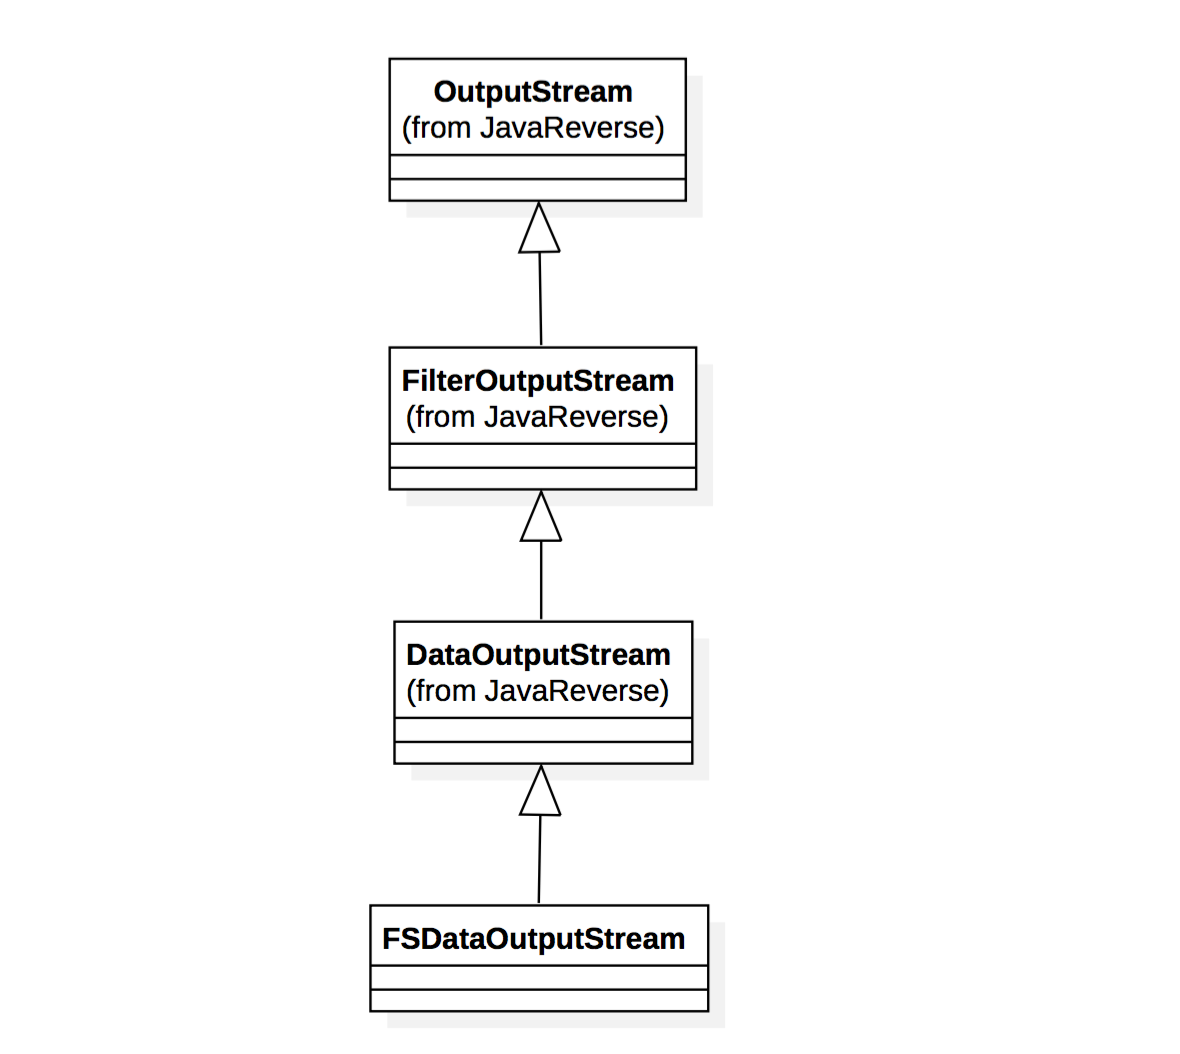
\includegraphics[width =1\linewidth]
{11.png}
\caption{outputstream 及其子类}
\label{fig:OutputStream}
\end{figure}

OutputStream

关闭此输出流并释放与此流相关联的任何系统资源。总的合同close 是关闭输出流。封闭流不能执行输出操作,无法重新打开。
该close方法OutputStream不执行任何操作。
\begin{java}
public void close()
\end{java}
刷新此输出流并强制任何缓冲的输出字节被写出。通常的合同flush是指出,如果以前写入的任何字节已经通过输出流的实现被缓冲,则这些字节应该立即被写入到它们的预定目的地。
如果此流的预期目标是由底层操作系统(例如文件)提供的抽象,那么刷新流仅保证先前写入流的字节传递到操作系统进行写入; 它并不保证它们实际上被写入物理设备,如磁盘驱动器。

该flush方法OutputStream不执行任何操作。
\begin{java}
public void flush()
\end{java}
len将从偏移量开始的指定字节数组的字节写入off此输出流。一般合同write(b, off, len)是数组b中的一些字节按顺序写入输出流; 元素b[off]是写入的第一个字节,b[off+len-1]是此操作写入的最后一个字节。
所述write的方法OutputStream被写出呼叫在每个字节中的一个参数的写入方法。鼓励子类覆盖此方法并提供更有效的实现。

如果b是null, NullPointerException则抛出一个。

如果off为负数,或len为负数,或 off+len大于数组的长度 b,则抛出IndexOutOfBoundsException。
\begin{java}
public void write(byte [] b,int off,int len)
\end{java}
将b.length指定字节数组的字节写入此输出流。总的合同write(b) 是它应该具有与通话完全相同的效果 write(b, 0, b.length)。
\begin{java}
public void write(byte [] b)
\end{java}
将指定的字节写入此输出流。一般的合同write是一个字节被写入输出流。要写入的字节是参数的8个低位b。24个高位b被忽略。
子类OutputStream必须为此方法提供一个实现。
\begin{java}
public abstract void write(int b)
\end{java}

FilterOutputStream

创建一个基于指定底层输出流的输出流过滤器。
参数:
out- 要分配给field.out以供以后使用的底层输出流,或者 null如果要创建此实例而不使用底层流。
\begin{java}
public FilterOutputStream(OutputStream  out)
\end{java}
将指定的数据写入byte此输出流。

所述write的方法FilterOutputStream 调用write它的基本输出流的方法,也就是说,它执行out.write(b)中。

实现抽象的写入方法的OutputStream。

\begin{java}
public void write(int b)
\end{java}
将b.length字节写入此输出流。

该write方法FilterOutputStream 调用其write与参数的三个参数的方法b,0和 b.length。

请注意,此方法不 write使用单个参数调用其基础流的单参数方法b。
\begin{java}
public void write(byte [] b)
\end{java}
len从指定的byte数组写入从 偏移量off到该输出流的字节。

所述write的方法FilterOutputStream 调用的write每个一个参数的方法 byte,以输出。

请注意,此方法不会write使用相同的参数调用其底层输入流的方法。子类FilterOutputStream应提供更有效的方法实现。

\begin{java}
public void write(byte [] b,int off,int len)
\end{java}

刷新此输出流,并强制将任何缓冲的输出字节写入流。

所述flush的方法FilterOutputStream 调用flush其基础输出流的方法。
\begin{java}
public void flush()
\end{java}
关闭此输出流并释放与流相关联的任何系统资源。

所述close的方法FilterOutputStream 的调用其flush的方法,然后调用 close它的基本输出流的方法。
\begin{java}
public void close()
\end{java}

DataOutputStream

创建一个新的数据输出流,以将数据写入指定的底层输出流。计数器written设置为零。

\begin{java}
public DataOutputStream(OutputStream  out)
\end{java}
将指定的字节(参数的低8位 b)写入底层输出流。如果没有异常抛出,计数器written将递增 1。

实现write方法OutputStream。
\begin{java}
public void write(int b)
\end{java}
len从指定的字节数组写入字节,从偏移开始off到底层输出流。如果没有异常抛出,计数器written将递增len。
\begin{java}
public void write(byte [] b,int off,int len)
\end{java}
刷新此数据输出流。这将强制任何缓冲的输出字节写入流。

所述flush的方法DataOutputStream 调用flush其基础输出流的方法。
\begin{java}
public void flush()
\end{java}

将boolean底层输出流写入1字节值。该值true作为值写出(byte)1; 该值false将作为值写出(byte)0。如果没有异常抛出,计数器written将递增 1。
\begin{java}
public final void writeBoolean(boolean v)
\end{java}
将byte底层输出流写入1字节值。如果没有异常抛出,计数器 written将递增1。
\begin{java}
public final void writeByte(int v)
\end{java}

将short底层输出流写入两个字节,高字节优先。如果没有异常抛出,计数器 written将递增2。
\begin{java}
public final void writeShort(int v)
\end{java}
将char底层输出流写入2字节值,先将高字节写入。如果没有异常抛出,计数器written将递增2。
\begin{java}
public final void writeChar(int v)
\end{java}
将int底层输出流写入四字节,高位字节。如果没有异常抛出,计数器 written将递增4。
\begin{java}
public final void writeInt(int v)
\end{java}

将long底层输出流写入八字节,高位字节。抛出任何异常,计数器 written增加8。
\begin{java}
public final void writeLong(long v)
\end{java}
将float参数转换为int使用floatToIntBits类中的 方法Float,然后将该int值写入底层输出流,为4字节数量,高字节为首。如果没有异常抛出,计数器written将递增4。

\begin{java}
public final void writeFloat(float v)
\end{java}

将double参数转换为long使用doubleToLongBits类中的 方法Double,然后将该long值作为8字节数量,高字节优先写入底层输出流。如果没有异常抛出,计数器written将递增8。

\begin{java}
public final void writeDouble(double v)
\end{java}

将字符串作为字节序列写入基础输出流。字符串中的每个字符顺序地通过丢弃其高8位来写出。如果没有异常被抛出,计数器written的长度就会增加s。
\begin{java}
public final void writeBytes(String  s)
\end{java}

将字符串写入底层输出流作为一系列字符。每个字符都被写入到数据输出流中,如同通过该writeChar方法一样。如果没有抛出异常,计数器written的长度增加两倍s。
\begin{java}
public final void writeChars(String  s)
\end{java}

使用修改的UTF-8 编码以机器无关方式将字符串写入底层输出流。

首先,将两个字节写入输出流,就像通过writeShort给出要跟随的字节数的 方法一样。该值是实际写出的字节数,而不是字符串的长度。按照长度,字符串的每个字符依次输出,使用修改的UTF-8编码字符。如果没有异常被抛出,计数器 written将增加写入输出流的总字节数。这将至少是两个加上长度str,最多两个加三倍的长度str。


\begin{java}
public final void writeUTF(String str)
\end{java}

返回计数器的当前值,written到目前为止写入此数据输出流的字节数。如果计数器溢出,它将被包装到Integer.MAX\_VALUE。
\begin{java}
public final int size()
\end{java}

FSDataOutputStream

\begin{figure}[h]
\centering
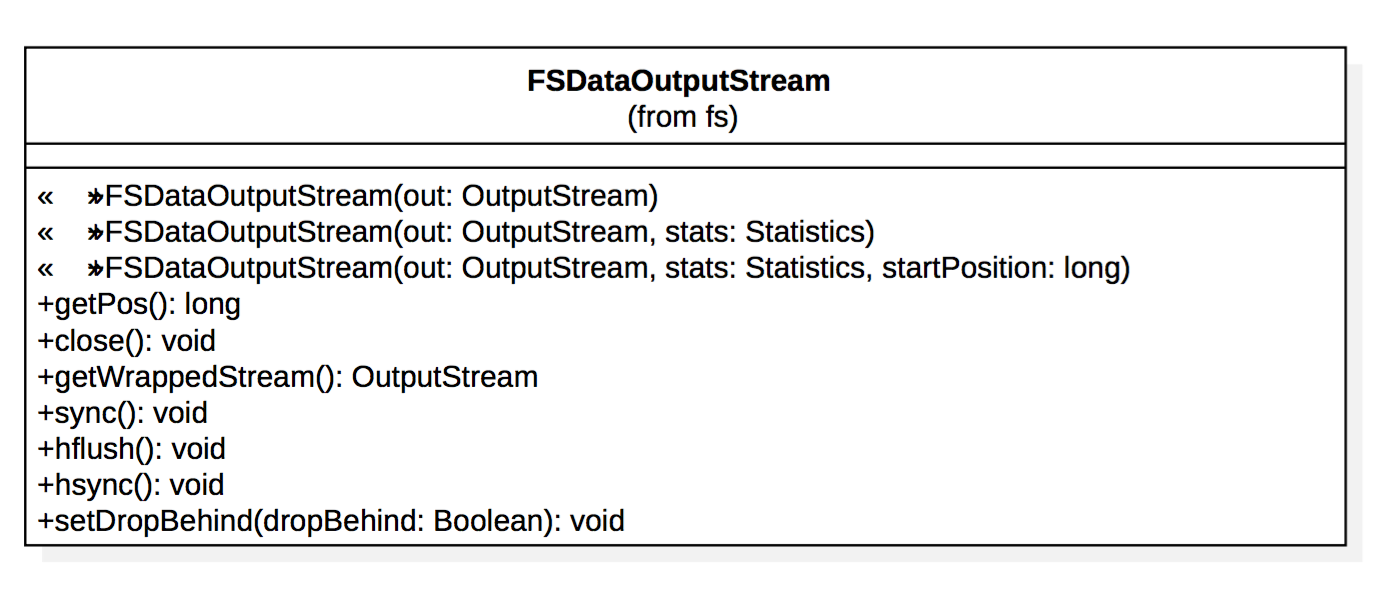
\includegraphics[width =1\linewidth]{1.png}
\caption{FSDataOutputStream}
\label{fig:FSDataOutputStream}
\end{figure}

\begin{figure}[h]
\centering
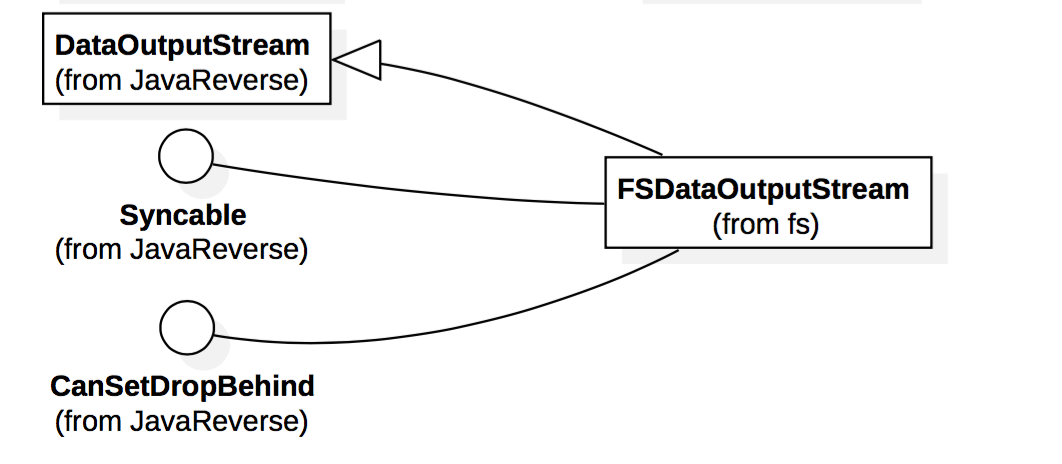
\includegraphics[width =1\linewidth]{2.png}
\caption{Hierarchy of FSDataOutputStream}
\label{fig:Hierarchy of FSDataOutputStream}
\end{figure}

Hadoop 的FileSystem中的create()方法返回了一个FSDataOutputStream对象。与FSDataInputStream一样,它也有一个用于查询位移的方法。但并没有类似于FSDataInputStream中seek()的方法,因为Hadoop不允许向流中的任意位置写数据,我们只能在一个文件的末尾处添加数据。同时2.8.0版本的Hadoop相较于旧版本,多实现了一个接口:CanSetDropBehind。

该接口声明了一个方法:
\begin{java}
public void setDropBehind(Boolean dropBehind) throws IOException
\end{java}
用于判断流是否应该丢弃缓存。

FSDataOutputStream同样实现了getPos()的功能:

\begin{java}
public long getPos() throws IOException
\end{java}
用于获取输入流的当前位置,并返回输入流的当前位置

继承关系:

java.lang.Object -->

java.io.OutputStream -->

java.io.FilterOutputStream -->

java.io.DataOutputStream -->

org.apache.hadoop.fs.FSDataOutputStream



FSDataOutputStream继承自DataOutputStream 并实现了接口Syncable和接口CanSetDropBehind,下面是对该类的具体说明:

三个构造函数:

该构造函数已过时
\begin{java}
@Deprecated
public FSDataOutputStream(OutputStream out) throws IOException {
	this(out, null);
}
\end{java}
该构造函数的参数包括:OutputStream类型的参数,Statistics类的参数
\begin{java}
public FSDataOutputStream(OutputStream out, FileSystem.Statistics stats)throws IOException {
	this(out, stats, 0);
}
\end{java}
该构造函数的参数包括:OutputStream类型的参数,Statistics类的参数和当前流的开始位置。
\begin{java}
public FSDataOutputStream(OutputStream out, FileSystem.Statistics stats,
		     long startPosition) throws IOException {
	super(new PositionCache(out, stats, startPosition));
	wrappedStream = out;
}
\end{java}
获取输入流的当前位置,并返回输入流的当前位置
\begin{java}
public long getPos() throws IOException {
	return position;
}

public long getPos() throws IOException {
	return ((PositionCache)out).getPos();
}
\end{java}
关闭基础输入流
\begin{java}
public void close() throws IOException {
	out.close();
}
\end{java}
刷新客户端中用户缓冲区的数据。在此调用的返回之后,新的读者将看到数据。来自于接口:Syncable
\begin{java}
public void hflush() throws IOException {
	if (wrappedStream instanceof Syncable) {
		((Syncable)wrappedStream).hflush();
    	} else {
      		wrappedStream.flush();
    }
}
\end{java}
将客户端用户缓冲区中的数据一直刷新到磁盘设备(但磁盘可能在其缓存中)。来自于接口:Syncable

\begin{java}
public void hsync() throws IOException {
	if (wrappedStream instanceof Syncable) {
      ((Syncable)wrappedStream).hsync();
	    } else {
      		wrappedStream.flush();
	}
}
\end{java}
配置判断流是否应该丢弃缓存。

参数:dropBehind:判断是否删除缓存

\begin{java}
public void setDropBehind(Boolean dropBehind) throws IOException {
	 try {
	    ((CanSetDropBehind)wrappedStream).setDropBehind(dropBehind);
	  } catch (ClassCastException e) {
	    throw new UnsupportedOperationException("the wrapped stream does " +
	        "not support setting the drop-behind caching setting.");
	  }
	}
\end{java}


\begin{figure}[h]
\centering
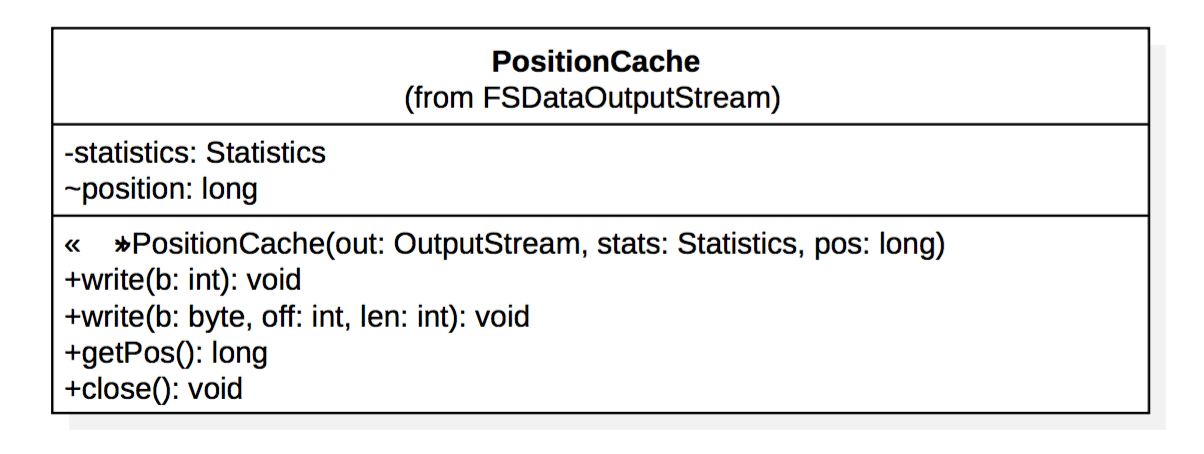
\includegraphics[width =1\linewidth]{3.png}
\caption{PositionCache}
\label{fig:PositionCache}
\end{figure}

FSDataOutputStream 中有一个内部类 PositionCache,其从 FilterOutputStream 派生,提供了缓
存文件指针 position 的功能,并且有一个 statistics 属性,用来统计。


接口:Syncable


\begin{java}
@InterfaceAudience.Public
@InterfaceStability.Evolving
public interface Syncable {
	 @Deprecated
	 public void sync() throws IOException;

	 public void hflush() throws IOException;

	 public void hsync() throws IOException;
}
\end{java}
接口:	CanSetDropBehind
\begin{java}
@InterfaceAudience.Public
@InterfaceStability.Evolving
public interface CanSetDropBehind {
	public void setDropBehind(Boolean dropCache)
	throws IOException, UnsupportedOperationException;
}
\end{java}
HDFS写文件过程
\begin{figure}[h]
\centering
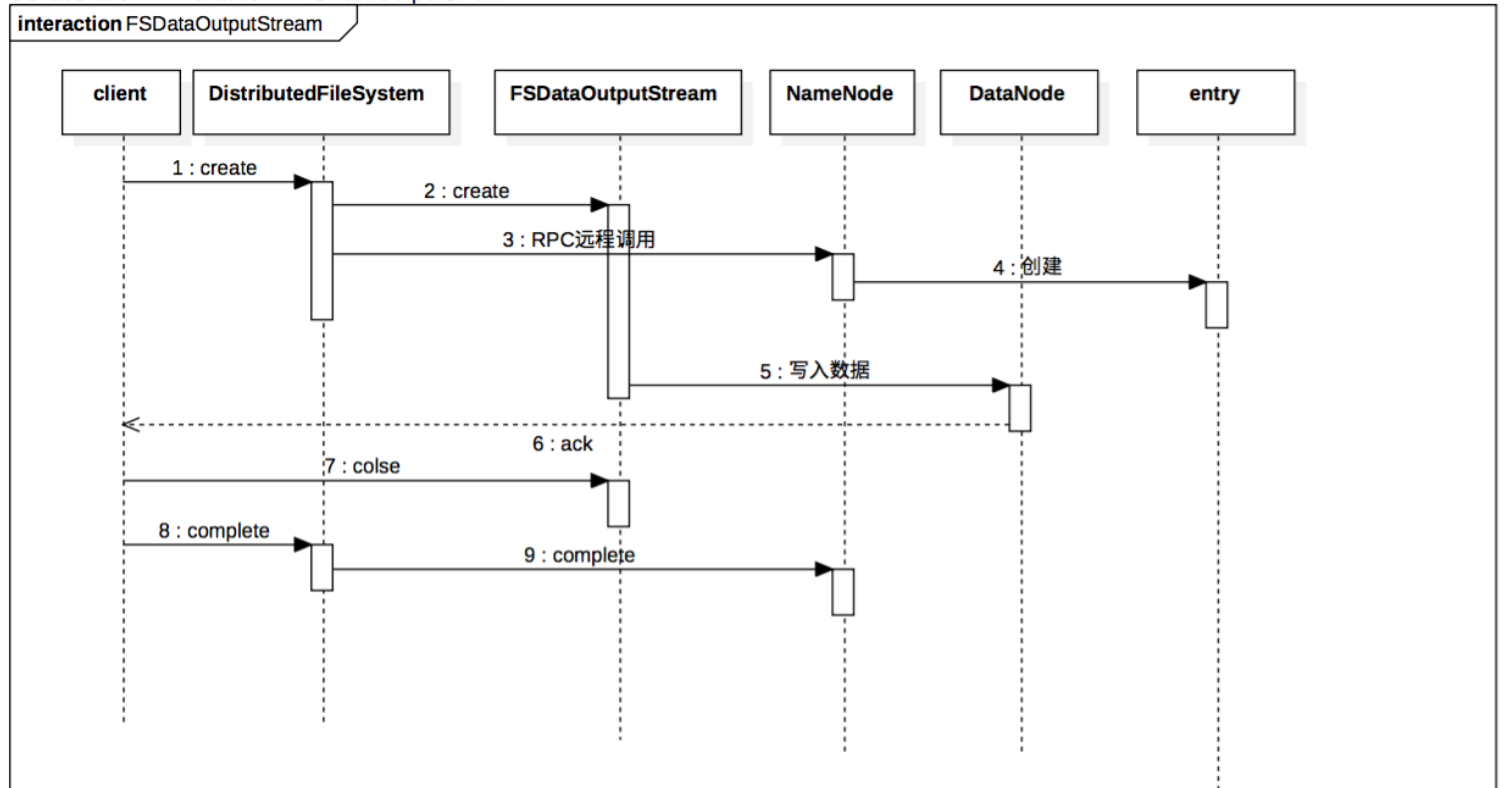
\includegraphics[width =1\linewidth]{write.png}
\caption{HDFS写文件时序图}
\label{fig:HDFS写文件时序图}
\end{figure}

Path

\begin{figure}[h]
\centering
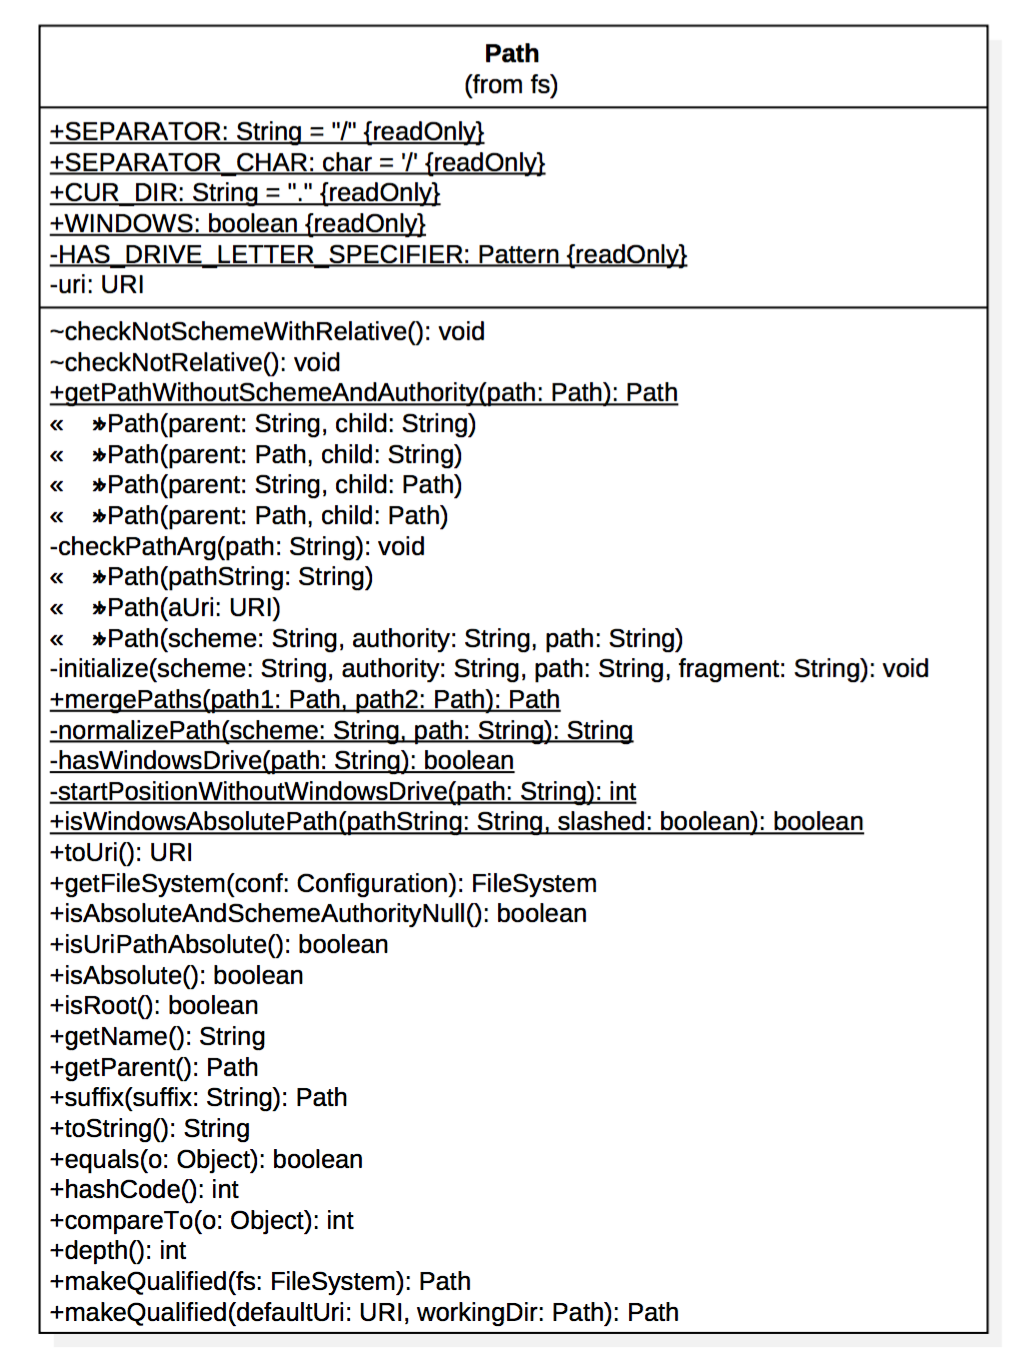
\includegraphics[width =1\linewidth]{6.png}
\caption{Path}
\label{fig:Path}
\end{figure}

\begin{figure}[h]
\centering
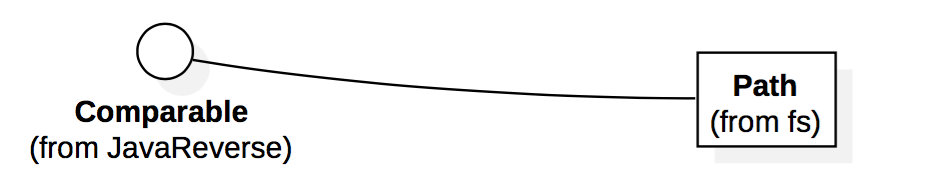
\includegraphics[width =1\linewidth]{7.png}
\caption{Hierarchy of Path}
\label{fig:Hierarchy of Path}
\end{figure}

在一个FileSystem中命名一个文件或目录。路径字符串使用斜杠作为目录分隔符。

Path 对路径进行解析,将参数转换为标准的URI格式,对Path的参数作判断,标准化,字符化等操作。
继承关系:

java.lang.Object -->

org.apache.hadoop.fs.Path


构造函数

基于根据父路径解析的子路径创建新路径。
\begin{java}
public Path(String parent, String child) {
	this(new Path(parent), new Path(child));
}
\end{java}
基于根据父路径解析的子路径创建新路径。
\begin{java}
public Path(Path parent, String child) {
	this(parent, new Path(child));
}
\end{java}
基于根据父路径解析的子路径创建新路径。
\begin{java}
public Path(String parent, Path child) {
	this(new Path(parent), child);
}
\end{java}
基于根据父路径解析的子路径创建新路径。
\begin{java}
public Path(Path parent, Path child) {
	  URI parentUri = parent.uri;
	  String parentPath = parentUri.getPath();
	  if (!(parentPath.equals("/") || parentPath.isEmpty())) {
	    try {
	      parentUri = new URI(parentUri.getScheme(), parentUri.getAuthority(),
	                    parentUri.getPath()+"/", null, parentUri.getFragment());
	    } catch (URISyntaxException e) {
	      throw new IllegalArgumentException(e);
	    }
	  }
	  URI resolved = parentUri.resolve(child.uri);
	  initialize(resolved.getScheme(), resolved.getAuthority(),
	             resolved.getPath(), resolved.getFragment());
	}
\end{java}
从组件构造路径。
\begin{java}
public Path(String scheme, String authority, String path) {
  checkPathArg( path );

  if (hasWindowsDrive(path) && path.charAt(0) != '/') {
    path = "/" + path;
  }

	if (!WINDOWS && path.charAt(0) != '/') {
    path = "./" + path;
  }

  initialize(scheme, authority, path, null);
}
\end{java}
\begin{java}
public int compareTo(Object o) {
  Path that = (Path)o;
  return this.uri.compareTo(that.uri);
}
\end{java}
返回此路径中的元素数。
\begin{java}
public int depth() {
  String path = uri.getPath();
  int depth = 0;
  int slash = path.length()==1 && path.charAt(0)=='/' ? -1 : 0;
  while (slash != -1) {
    depth++;
    slash = path.indexOf(SEPARATOR, slash+1);
	}
	return depth;
}
\end{java}
返回拥有此路径的文件系统。
\begin{java}
public FileSystem getFileSystem(Configuration conf) throws IOException {
  return FileSystem.get(this.toUri(), conf);
}
\end{java}
返回此路径的最终组件。
\begin{java}
public String getName() {
  String path = uri.getPath();
  int slash = path.lastIndexOf(SEPARATOR);
  return path.substring(slash+1);
}
\end{java}
返回路径的父亲, 如果为根, 则为 null。
\begin{java}
public Path getParent() {
  String path = uri.getPath();
  int lastSlash = path.lastIndexOf('/');
  int start = startPositionWithoutWindowsDrive(path);
  if ((path.length() == start) ||               // empty path
      (lastSlash == start && path.length() == start+1)) { // at root
    return null;
  }
	String parent;
  if (lastSlash==-1) {
    parent = CUR_DIR;
  } else {
    parent = path.substring(0, lastSlash==start?start+1:lastSlash);
  }
  return new Path(uri.getScheme(), uri.getAuthority(), parent);
}
\end{java}
返回给定路径的版本, 而不提供方案信息。
\begin{java}
public static Path getPathWithoutSchemeAndAuthority(Path path) {
  Path newPath = path.isUriPathAbsolute() ?
    new Path(null, null, path.toUri().getPath()) :
    path;
  return newPath;
}
\end{java}
返回路径组件
\begin{java}
public boolean isAbsolute() {
   return isUriPathAbsolute();
}
\end{java}
\begin{java}
public boolean isAbsoluteAndSchemeAuthorityNull() {
  return  (isUriPathAbsolute() &&
      uri.getScheme() == null && uri.getAuthority() == null);
}
\end{java}
\begin{java}
public boolean isUriPathAbsolute() {
  int start = startPositionWithoutWindowsDrive(uri.getPath());
  return uri.getPath().startsWith(SEPARATOR, start);
}
\end{java}

如果且仅当此路径表示文件系统的根, 则返回 true。
\begin{java}
public boolean isRoot() {
  return getParent() == null;
}
\end{java}
确定给定的路径字符串是否表示 windows 上的绝对路径。
\begin{java}
public static boolean isWindowsAbsolutePath(final String pathString,
                                            final boolean slashed) {
  int start = startPositionWithoutWindowsDrive(pathString);
  return start > 0
      && pathString.length() > start
      && ((pathString.charAt(start) == SEPARATOR_CHAR) ||
          (pathString.charAt(start) == '\\'));
}
\end{java}
\begin{java}
public Path makeQualified(URI defaultUri, Path workingDir ) {
  Path path = this;
  if (!isAbsolute()) {
    path = new Path(workingDir, this);
  }

  URI pathUri = path.toUri();

  String scheme = pathUri.getScheme();
  String authority = pathUri.getAuthority();
  String fragment = pathUri.getFragment();

  if (scheme != null &&
      (authority != null || defaultUri.getAuthority() == null))
    return path;
  if (scheme == null) {
    scheme = defaultUri.getScheme();
  }

  if (authority == null) {
    authority = defaultUri.getAuthority();
    if (authority == null) {
      authority = "";
    }
  }
  URI newUri = null;
  try {
    newUri = new URI(scheme, authority ,
      normalizePath(scheme, pathUri.getPath()), null, fragment);
  } catch (URISyntaxException e) {
    throw new IllegalArgumentException(e);
  }
  return new Path(newUri);
}
\end{java}
合并两路径, 使第二个路径相对于第一个路径被追加
\begin{java}
public static Path mergePaths(Path path1, Path path2) {
  String path2Str = path2.toUri().getPath();
  path2Str = path2Str.substring(startPositionWithoutWindowsDrive(path2Str));
  return new Path(path1.toUri().getScheme(),
      path1.toUri().getAuthority(),
      path1.toUri().getPath() + path2Str);
}
在路径中的最终名称中添加一个后缀。
\begin{java}
public Path suffix(String suffix) {
  return new Path(getParent(), getName()+suffix);
}
\end{java}
将此路径转换为 uri。
\begin{java}
public URI toUri() { return uri; }
\end{java}

QuotaUsage

\begin{figure}[h]
\centering
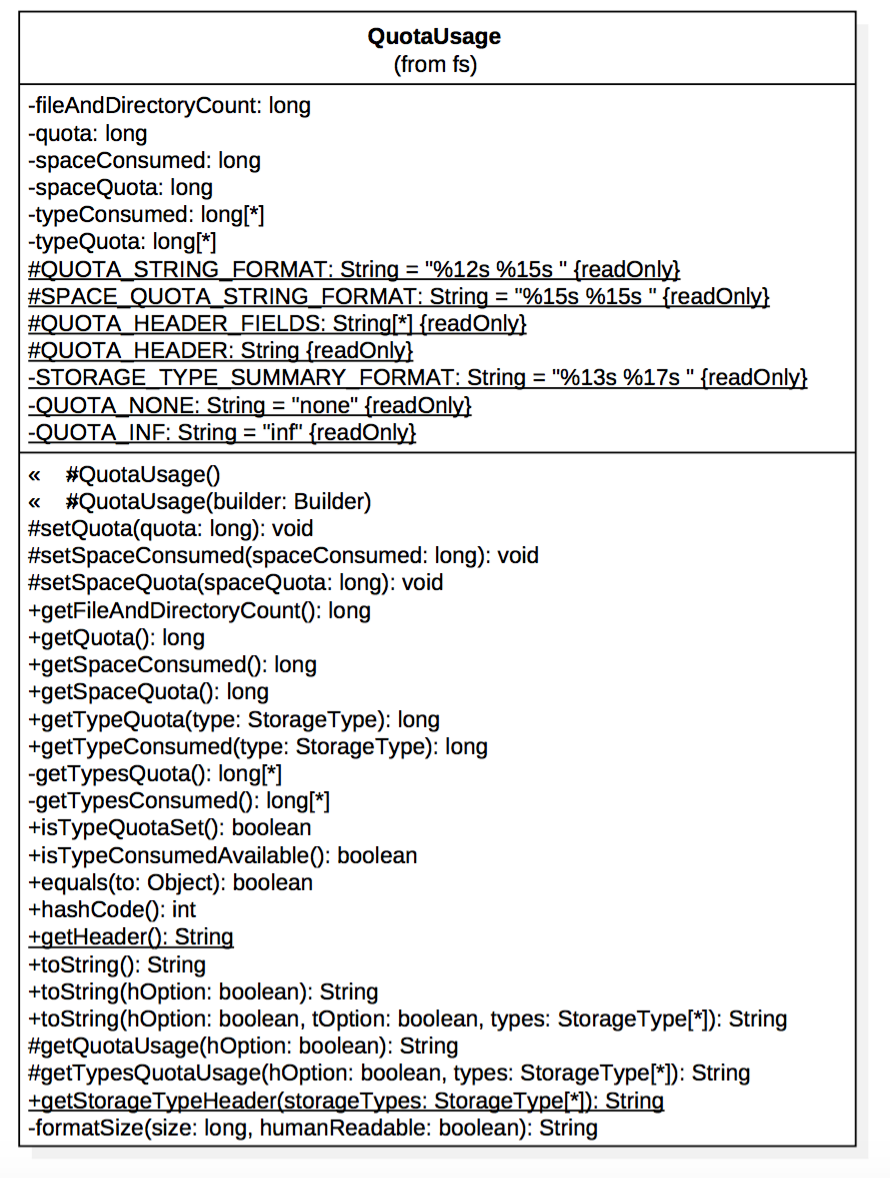
\includegraphics[width =1\linewidth]{8.png}
\caption{QuotaUsage}
\label{fig:QuotaUsage}
\end{figure}

存储目录的配额分配情况。

Quota有以下三种:

Name Quotas : 限制某个目录下的文件和文件夹数量

Space Quotas : 设置某个目录的空间大小

Type Quotas : 设置某个目录的类型数量

fileAndDirectoryCount:文件和目录数量

quota:命名空间的quota(限制文件数)

spaceQuota:物理空间的quota (限制磁盘空间占用大小)

spaceConsumed:消耗的物理空间

typeQuota:类型的quota(限制类型数)

typeConsumed:消耗的类型数

返回输出的标头。
\begin{java}
public static String getHeader() {
  return QUOTA_HEADER;
}
\end{java}
返回目录配额
\begin{java}
public long getQuota() {
  return quota;
}
\end{java}
返回已消耗的(磁盘)空间
\begin{java}
public long getSpaceConsumed() {
  return spaceConsumed;
}
\end{java}
返回 (磁盘) 空间配额。
\begin{java}
public long getSpaceQuota() {
  return spaceQuota;
}
\end{java}
返回 StorageTypes 的标题。
\begin{java}
public static String getStorageTypeHeader(List<StorageType> storageTypes) {
  StringBuffer header = new StringBuffer();

  for (StorageType st : storageTypes) {
    String storageName = st.toString();
    header.append(String.format(STORAGE_TYPE_SUMMARY_FORMAT,
        storageName + "_QUOTA", "REM_" + storageName + "_QUOTA"));
  }
  return header.toString();
}
\end{java}
返回消耗的存储类型。
\begin{java}
public long getTypeConsumed(StorageType type) {
  return (typeConsumed != null) ? typeConsumed[type.ordinal()] : 0;
}
\end{java}
返回消耗的类型配额
\begin{java}
public long getTypeQuota(StorageType type) {
  return (typeQuota != null) ? typeQuota[type.ordinal()] : -1;
}
\end{java}
如果有任何存储类型的消耗信息可用, 则返回 true。
\begin{java}
public boolean isTypeConsumedAvailable() {
  if (typeConsumed == null) {
    return false;
  }
  for (StorageType t : StorageType.getTypesSupportingQuota()) {
    if (typeConsumed[t.ordinal()] > 0) {
      return true;
    }
  }
  return false;
}
\end{java}
如果有任何存储类型配额已被设置, 则返回 true。
\begin{java}
public boolean isTypeQuotaSet() {
  if (typeQuota == null) {
    return false;
  }
  for (StorageType t : StorageType.getTypesSupportingQuota()) {
    if (typeQuota[t.ordinal()] > 0) {
      return true;
    }
  }
  return false;
}
\end{java}

ContentSummary

\begin{figure}[h]
\centering
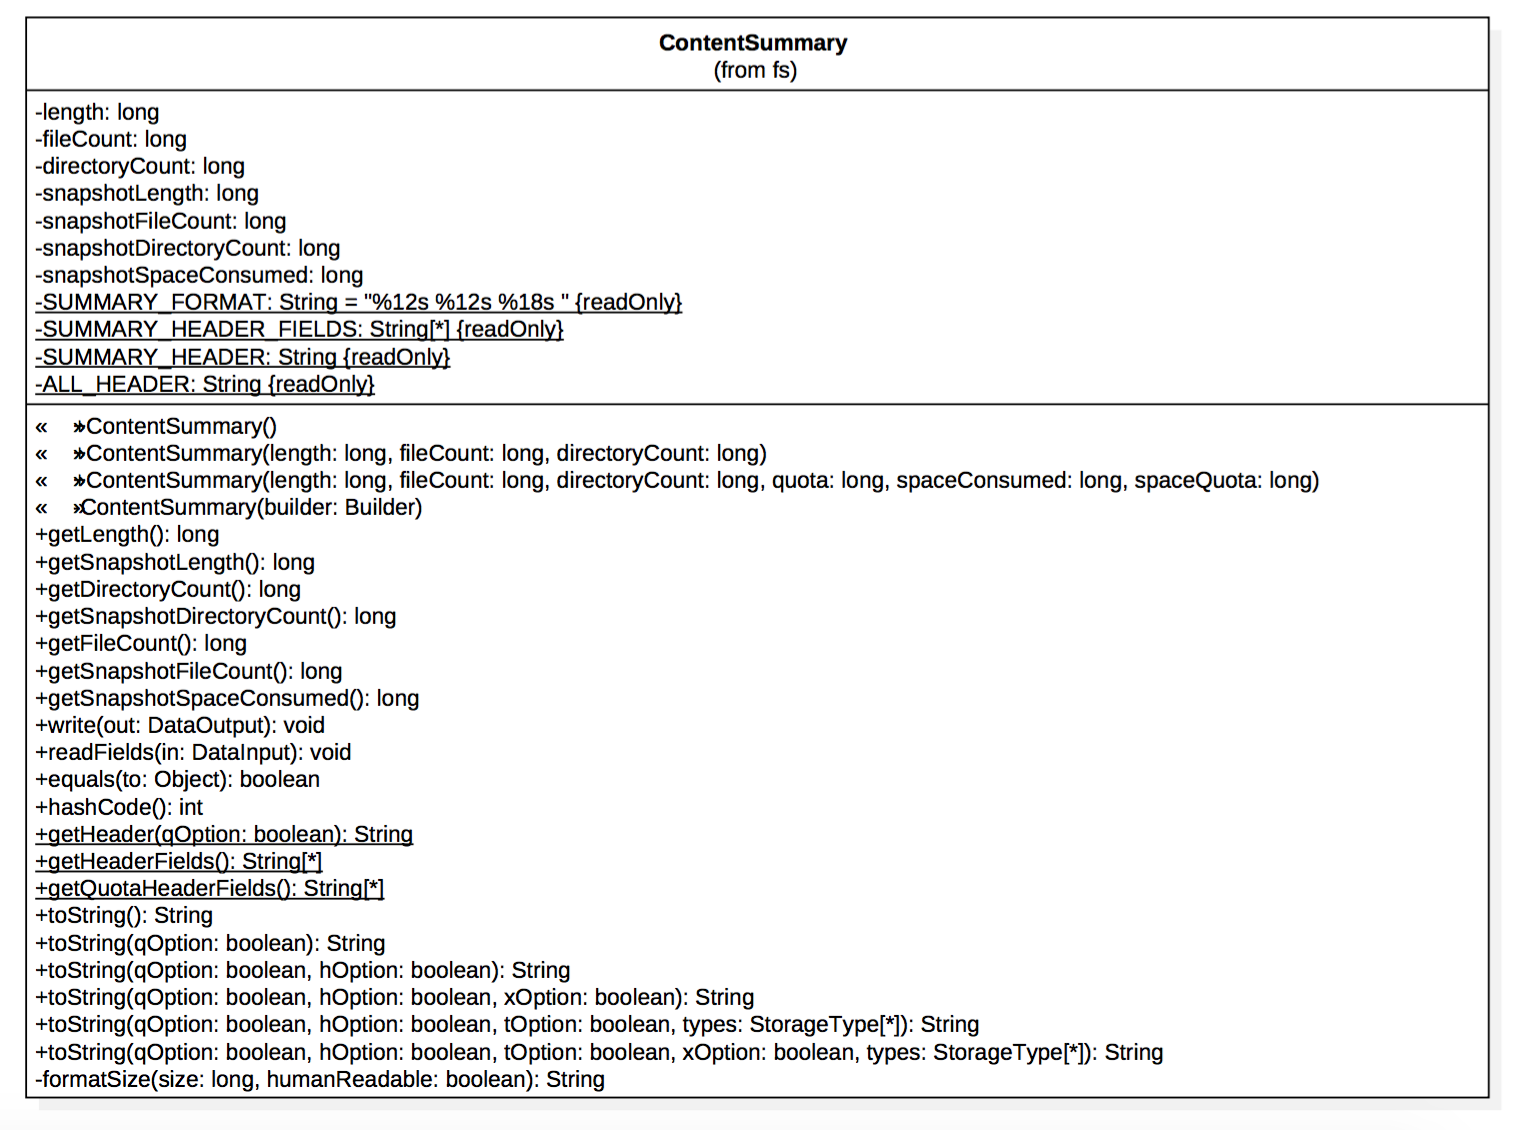
\includegraphics[width =1\linewidth]{9.png}
\caption{ContentSummary}
\label{fig:ContentSummary}
\end{figure}

\begin{figure}[h]
\centering
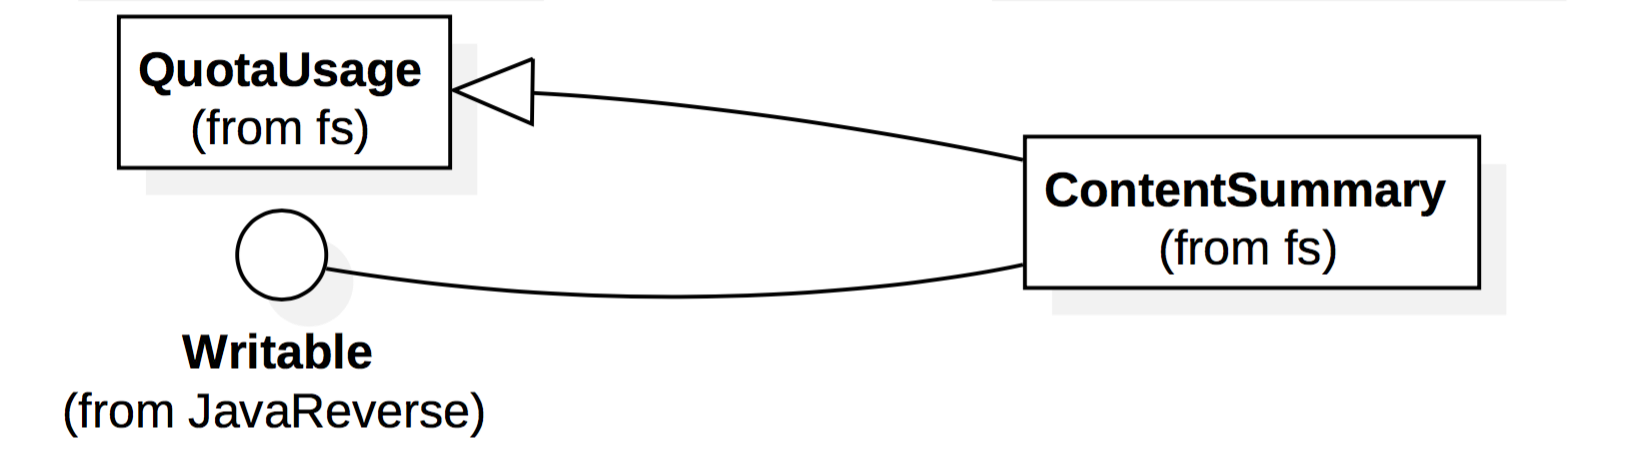
\includegraphics[width =1\linewidth]{10.png}
\caption{Hierarchy of ContentSummary}
\label{fig:Hierarchy of ContentSummary}
\end{figure}

ContentSummary 存储内容(目录或文件)的摘要。

类存储有关文件或目录的一些信息,包括文件长度,文件数量,目录数量,
磁盘配额,已用空间大小,剩余空间大小。

构造函数
\begin{java}
private ContentSummary(Builder builder) {
  super(builder);
  this.length = builder.length;
  this.fileCount = builder.fileCount;
  this.directoryCount = builder.directoryCount;
  this.snapshotLength = builder.snapshotLength;
  this.snapshotFileCount = builder.snapshotFileCount;
  this.snapshotDirectoryCount = builder.snapshotDirectoryCount;
  this.snapshotSpaceConsumed = builder.snapshotSpaceConsumed;
}
\end{java}
返回输出的标题。如果qOption为false,输出目录数,文件数和内容大小; 如果qOption为真,则输出配额和剩余配额
\begin{java}
public static String getHeader(boolean qOption) {
  return qOption ? ALL_HEADER : SUMMARY_HEADER;
}
\end{java}
从摘要标题返回字段的名称。
\begin{java}
public static String[] getHeaderFields() {
  return SUMMARY_HEADER_FIELDS;
}
\end{java}
返回配额摘要中使用的字段的名称。
\begin{java}
public static String[] getQuotaHeaderFields() {
  return QUOTA_HEADER_FIELDS;
}
\end{java}
以输出格式返回对象的字符串表示形式。如果qOption为false,输出目录数,文件数和内容大小; 如果qOption为真,则输出配额和剩余配额。
\begin{java}
public String toString(boolean qOption) {
  return toString(qOption, false);
}
\end{java}
以输出格式返回对象的字符串表示形式。

参数:

qOption - 指示是否需要打印配额的标志

hOption - 一个标志,指示是否使用可读的输出


返回:
对象的字符串表示形式
\begin{java}
public String toString(boolean qOption, boolean hOption) {
  return toString(qOption, hOption, false, null);
}
\end{java}
以输出格式返回对象的字符串表示形式。

参数:

qOption - 指示是否需要打印配额的标志

hOption - 指示是否使用人类可读输出的标志

xOption - 一个标志,指示从快照计算是否包括在输出中

返回:

对象的字符串表示形
\begin{java}
public String toString(boolean qOption, boolean hOption, boolean xOption) {
  return toString(qOption, hOption, false, xOption, null);
}
\end{java}
以输出格式返回对象的字符串表示形式。

参数:

qOption - 指示是否需要打印配额的标志

hOption - 一个标志,指示是否使用可读的输出

tOption - 表示存储类型是否显示配额的标志

types - 要显示的存储类型

返回:

对象的字符串表示形式

\begin{java}
public String toString(boolean qOption, boolean hOption,
                       boolean tOption, List<StorageType> types) {
  return toString(qOption, hOption, tOption, false, types);
}
\end{java}
以输出格式返回对象的字符串表示形式。

如果qOption为false,输出目录数,文件数和内容大小; 如果qOption为真,则输出配额和剩余配额。如果hOption为false,如果hOption为true,则以字节为单位返回文件大小,如果tOption为true,则文件大小返回为人类可读取,如果tOption为false,则显示存储类型的配额,与#toString(boolean,boolean)相同的逻辑if xOption为false,如果xOption为真,则输出包括从快照计算,输出不包括快照中的计算。

参数:

qOption - 指示是否需要打印配额的标志

hOption - 指示是否使用人类可读输出的标志

tOption - 表示存储类型是否显示配额的标志

xOption - 一个标志,指示从快照计算是否包括在输出中

types - 要显示的存储类型

返回:

对象的字符串表示形式

\begin{java}
public String toString(boolean qOption, boolean hOption, boolean tOption,
    boolean xOption, List<StorageType> types) {
  String prefix = "";
  if (tOption) {
    return getTypesQuotaUsage(hOption, types);
  }

  if (qOption) {
    prefix = getQuotaUsage(hOption);
  }

  if (xOption) {
    return prefix + String.format(SUMMARY_FORMAT,
        formatSize(directoryCount - snapshotDirectoryCount, hOption),
        formatSize(fileCount - snapshotFileCount, hOption),
        formatSize(length - snapshotLength, hOption));
  } else {
    return prefix + String.format(SUMMARY_FORMAT,
        formatSize(directoryCount, hOption),
        formatSize(fileCount, hOption),
        formatSize(length, hOption));
  }
}
\end{java}
FSOutputSummer
\begin{figure}[h]
\centering
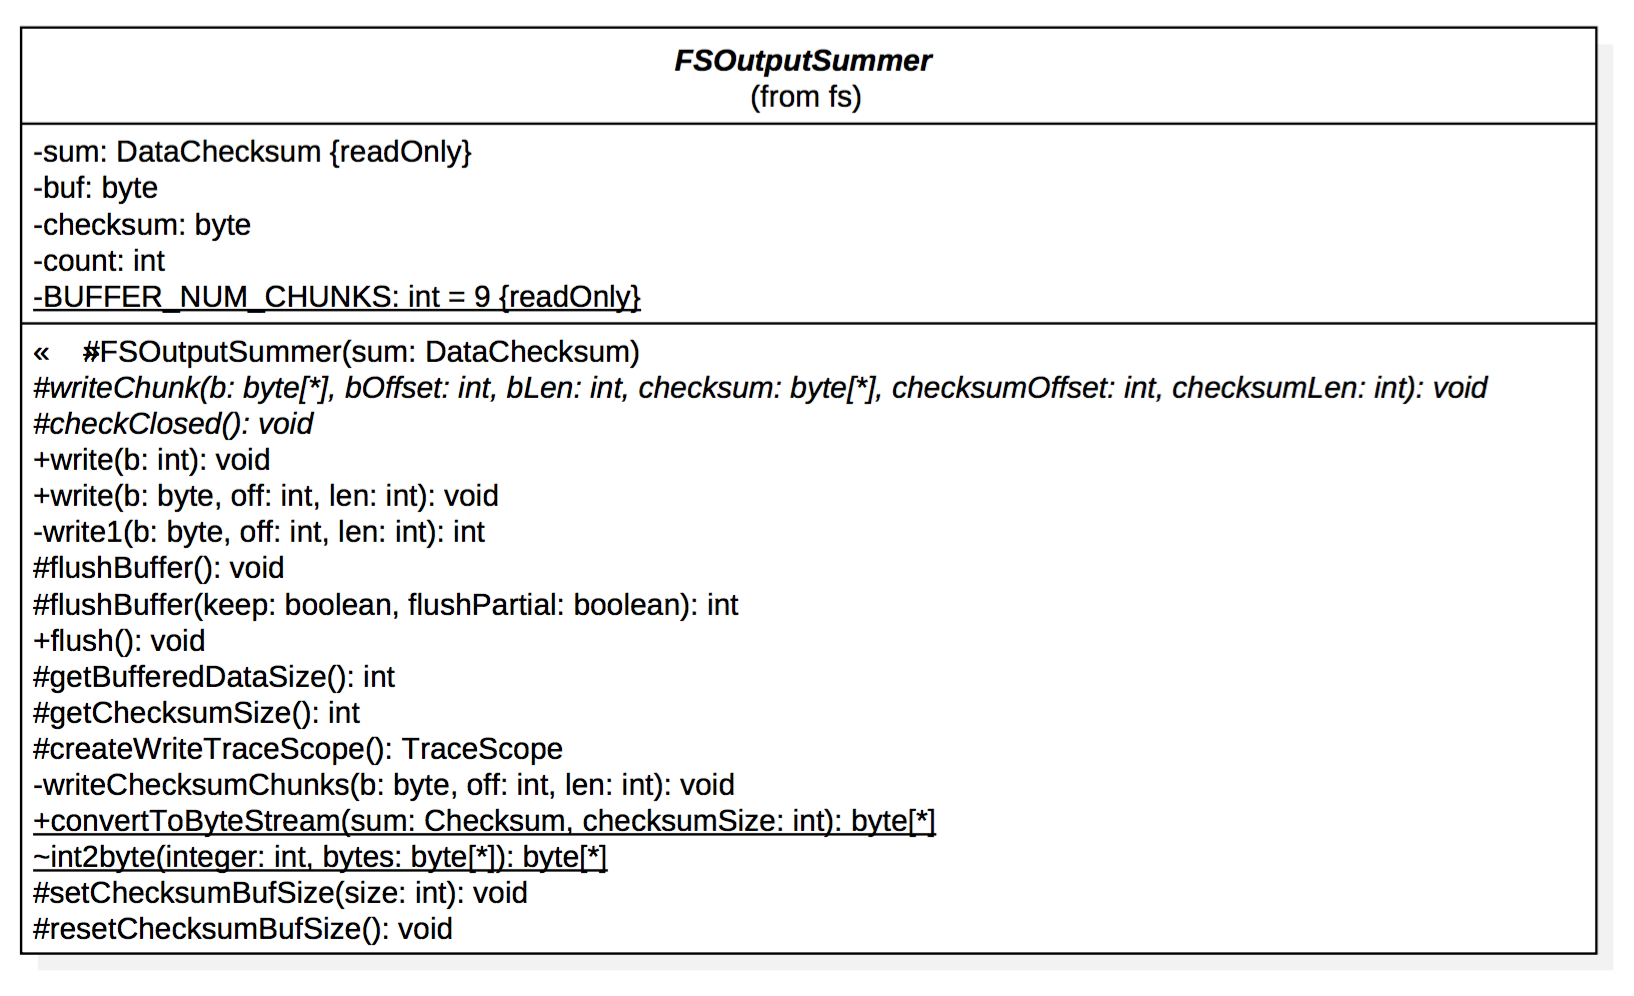
\includegraphics[width =1\linewidth]{4.png}
\caption{FSOutputSummer}
\label{fig:FSOutputSummer}
\end{figure}

\begin{figure}[h]
\centering
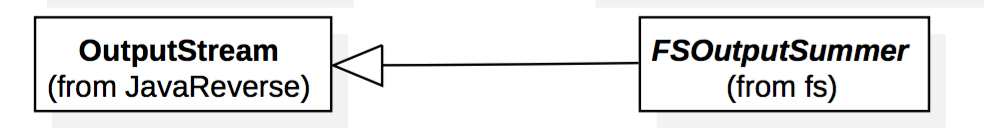
\includegraphics[width =1\linewidth]{5.png}
\caption{Hierarchy of FSOutputSummer}
\label{fig:Hierarchy of FSOutputSummer}
\end{figure}

构造函数:
\begin{java}
protected FSOutputSummer(DataChecksum sum) {
  this.sum = sum;
  this.buf = new byte[sum.getBytesPerChecksum() * BUFFER_NUM_CHUNKS];
  this.checksum = new byte[getChecksumSize() * BUFFER_NUM_CHUNKS];
  this.count = 0;
}
\end{java}

\endinput
